\documentclass{beamer}
\usepackage[T2A]{fontenc}
\usepackage[utf8]{inputenc}
\usepackage[english,russian]{babel}
\usepackage{amssymb,amsfonts,amsmath,mathtext}
\usepackage{cite,enumerate,float,indentfirst}
\usepackage[dvips]{graphicx}
\usepackage[linesnumbered,ruled,vlined]{algorithm2e} % NEW

\setbeamertemplate{footline}[page number]

\title[\insertframenumber/\inserttotalframenumber]
{Метод извлечения семантических отношений из разнородных источников текстовой информации }

\author[Александр Панченко]
{Александр Панченко, Аспирант МГТУ им. Н.Э. Баумана и Catholic Univeristy of Louvain \\ {\scriptsize \url{alexander.panchenko@student.uclouvain.be} }}

\AtBeginSubsection[]
{
  \begin{frame}<beamer>
    \frametitle{Plan}
    \tableofcontents[currentsection,currentsubsection]
  \end{frame}
}


\mode<presentation>
{
%\usetheme{Warsaw}
\usetheme{Singapore}
\usecolortheme{orchid}%whale
\useoutertheme{smoothbars}
%\usefonttheme{serif}
}

\setbeamertemplate{navigation symbols}{%
}

\begin{document}

\begin{frame}
  \titlepage
\end{frame}

\begin{frame}
  \setcounter{tocdepth}{1}
  \frametitle{Plan}
  \tableofcontents
  \setcounter{tocdepth}{2}
	
\end{frame}

\section{Введение}

\begin{frame}
\frametitle{Семантические отношения}
В рамках данной работы под семантическими отношениями понимаются: 
\begin{itemize}
\item \textbf{синонимы} (отношения эквивалентности): $\langle car,SYN,vehicle \rangle, \langle animal,SYN,beast \rangle$ 
\item \textbf{гиперонимы} (иерархические отношения): $\langle car,HYPER,Jeep \text{ } Cherokee \rangle, \langle animal,HYPER, crocodile \rangle$
\item \textbf{ко-гиперонимы} (общий гипероним):
$\langle Toyota \text{ } Land  \text{ }Cruiser,COHYPER,Jeep \text{ } Cherokee \rangle$
\end{itemize}

Формально:
\begin{itemize}
	
		\item $r=\left\langle   c_i,t,c_j \right\rangle$ -- \textbf{семантическое отношение},  где $c_i,c_j \in C$ -- \textbf{слова}, такие как \textit{radio} или \textit{receiver operating characteristic},  $t \in T$ -- \textbf{тип семантического отношения}, такой как \textit{синонимия} или \textit{гипонимия}
	\item  $R \subseteq C \times T \times C$ -- множество \textbf{семантических отношений} 
	\item  $R \subseteq C \times C$ -- множество \textbf{нетипизированных отношений} 
	
\end{itemize}

\end{frame}

%%%%%%%%%%%%%%%%%%%%%%%%%%%%%%%%%%%%%%%%%%%%%%%%%
\begin{frame}
\frametitle{Семантические отношения фиксируются в \ldots}

\textbf{Тезаурусах:} граф $G = (C,R)$

\begin{figure}	
	\centering
		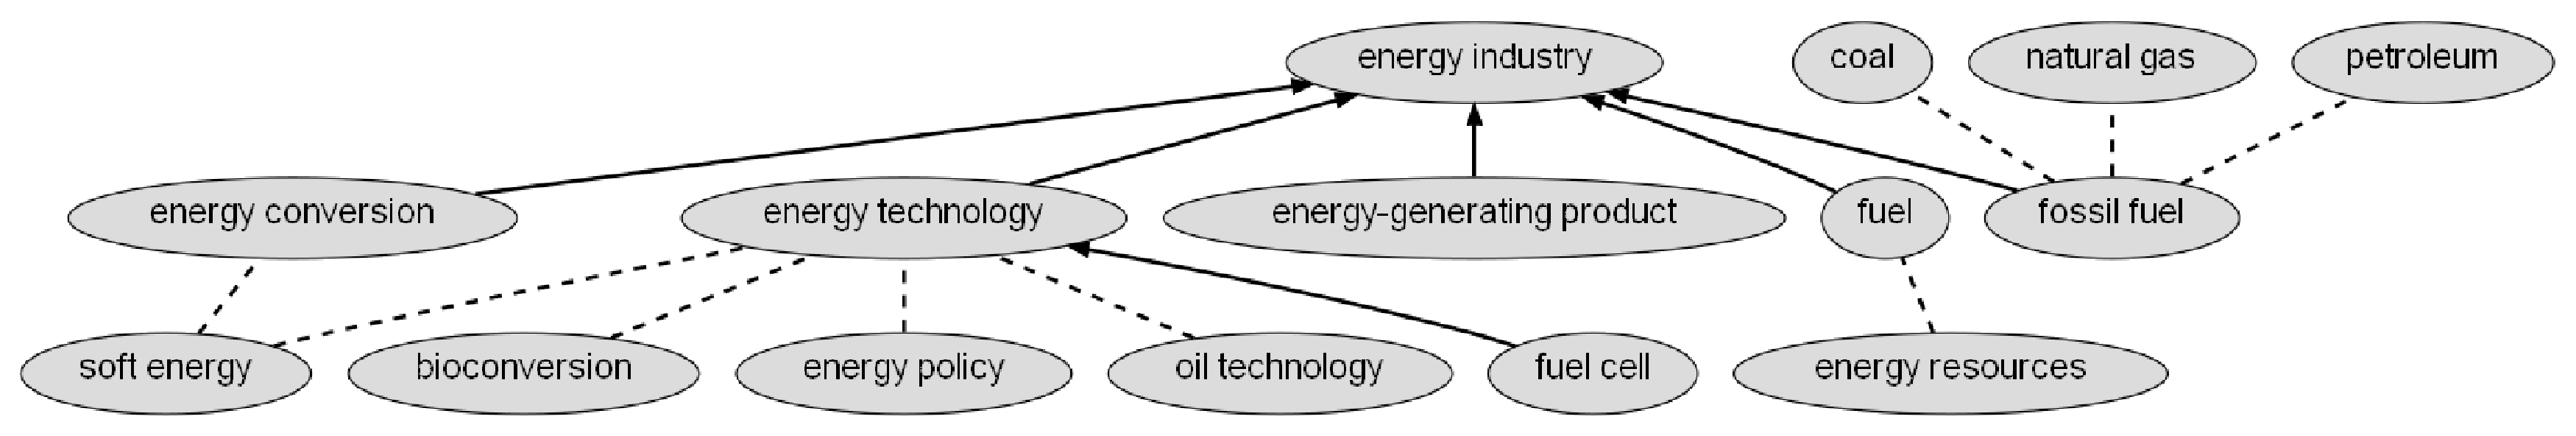
\includegraphics[width=1.0\textwidth]{figures/thesaurus2}
		\caption{Часть информационно-поискового тезуаруса EuroVoc.}
\end{figure}

\textbf{$T = \{NT, RT, USE\}$}

\textbf{$R=$}

\begin{itemize}
	\item $\left\langle   \text{energy-generating product, NT, energy industry} \right\rangle$
	\item $\left\langle   \text{energy technology, NT, energy industry} \right\rangle$
	\item $\left\langle   \text{petrolium, RT, fossil fuel} \right\rangle$
	%\item $\left\langle   \text{energy technology, RT, oil technology} \right\rangle$, \ldots
\end{itemize}

\textbf{Других семантических ресурсах:} онтологии, семантические сети, словари синонимов, терминологические классификаторы и т.п.

\end{frame}

%%%%%%%%%%%%%%%%%%%%%%%%%%%%%%%%%%%%%%%%%%%%%%%%%
\begin{frame}
\frametitle{Применение семантических отношений}
Семантические отношения представляют \textbf{знание о языке} полезное для различных приложений \textbf{автоматической обработки текста} (АОТ):
\begin{itemize}
  \item Расширение и рекомендация поискового запроса в ИПС (Hsu et al., 2006)
  \item Построение вопросно-ответных систем (Sun et al., 2005)	
  \item Категоризация текстовых документов (Tikk et al, 2003)
  \item Разрешение омонимии (Patwardhan et al., 2003)
  
	\end{itemize}
	
	В нашем случае:
	\begin{itemize}
	  \item Расширение поискового запроса
	  \item Построение классификатора имен файлов
	\end{itemize}

\end{frame}

%%%%%%%%%%%%%%%%%%%%%%%%%%%%%%%%%%%%%%%%%%%%%%%%%
\begin{frame}
\frametitle{Проблема}

\begin{itemize}
  \item Cуществующие ресурсы часто \textbf{недоступны или недостаточны} для
  \begin{itemize}
   \item конкретного приложения
   \item предметной области
   \item языка
  \end{itemize}
  \begin{block}{\textbf{Пример:} магазин продающий книги}
  \begin{figure}
	\centering
		
\includegraphics[width=0.18\textwidth]{figures/gof}

\end{figure}
	
   ``Design Patterns: Elements of Reusable Object-Oriented Software'' $\Leftrightarrow$ ``Gang of Four Book'' $\Leftrightarrow$ GOF
   
    \end{block}
    \item Как выдать в результате поиска книгу по запросу ``GOF''?
\end{itemize}
		
\end{frame}

\begin{frame}
\frametitle{Проблема}

\begin{itemize}
\item \textbf{Ручное создание требуемых семантических ресурсов}:
\begin{itemize}
\item (+) Точный результат 
\item (--) Крайне дорогостоящий и трудоемкий процесс
\item (--) Неприменимо в большом количестве случаев
\end{itemize}

\item Существующие методы извлечение отношений:
\begin{itemize}
  \item (--) Не обеспечивают достаточной точности  
  \end{itemize}

\item Поэтому, актуальной задачей является разработка методов автоматического извлечения семантических отношений:

\end{itemize}

\begin{block}{Метод извлечения семантических отношений}
\textbf{Вход:} слова $C$, типы семантических отношений $T$

\textbf{Выход:} семантические отношения $\hat{R}$, достоверность отношений $P(r) \in [0;1], \forall r \in R$.  
\end{block}

\end{frame}


%%%%%%%%%%%%%%%%%%%%%%%%%%%%%%%%%%%%%%%%%%%%%%%%%
\begin{frame}
\frametitle{Проблема: cуществующие методы извлечения отношений}

Основанны на \ldots 
\begin{itemize}
\item \textbf{лексико-синтаксических шаблонах} (Snow, 2004)
\item \textbf{корпусе текстов} (Филиппович и Прохоров, 2002; Grefenstette, 1994; Curran and Moens, 2002)
\item \textbf{определениях из словарей/энциклопедий} (Zesch, 2006)
\item \textbf{семантических сетях} (Pedersen, 2004)
\item \textbf{фолксономиях} (Markovich and Gabrilovich, 2006)
\item \textbf{подобии формы слов} (Левеншнейн)
\item \textbf{структуре гиперссылок документов} (Nakayama et al., 2007) 
\item \textbf{логах поисковых запросов} (Baezo-Yates, 2007)

\end{itemize}

\end{frame}

%%%%%%%%%%%%%%%%%%%%%%%%%%%%%%%%%%%%%%%%%%%%%%%%%%
\begin{frame}
\frametitle{Проблема: cуществующие методы}
\textbf{Состояние исследований и разработок}: 
\begin{itemize}
\item Существует \textbf{множество разнородных} методов извлечения, предоставляющих \textbf{взаимодополняющую информацию}.
\item Мы предлагаем \textbf{комбинацию} методов для улучшения результатов.
\end{itemize}


\textbf{Цели исследования}: 
\begin{itemize}
\item Какой базовый метод извлечения является наилучшим?
\item Как \textbf{эффективно комбинировать} методы для улучшения качества извлечения?
\end{itemize}
\end{frame}


%%%%%%%%%%%%%%%%%%%%%%%%%%%%%%%%%%%%%%%%%%%%%%%%%
\section{Метод}

\begin{frame}
\frametitle{Извлечение отношений на основе мер подобия}

\textbf{Решение:}
\begin{enumerate}
\item Представить результаты каждого $k$-го метода извлечения как метрику подобия $sim_k:C \times C \rightarrow [0;1]$.
\begin{itemize}
   
  \item $sim_k(c_i,c_j)$ -- семантическая близость $c_i$ и $c_j$. 
  \item $sim_k(x,y) = 1 \text{ тогда и только тогда, когда } x=y=c_i$
  \item $sim_k(c_i,c_j) = sim_k(c_j,c_i)$
  \item $sim_k(c_i,c_j) \leq sim_k(c_i,c_k) + sim_k(c_k,c_j)$
\end{itemize}
\item Комбинировать $N$ метрик в $sim_{cmb}$ с помощью метода комбинирования $combination\_method(sim_1, sim_2,\ldots,sim_N) \rightarrow [0;1]$
\item Вычислить отношения на основе $sim_{cmb}$.
\end{enumerate}

\end{frame}

\begin{frame}
\frametitle{Извлечение отношений на основе мер подобия}

\begin{figure}
	\centering
		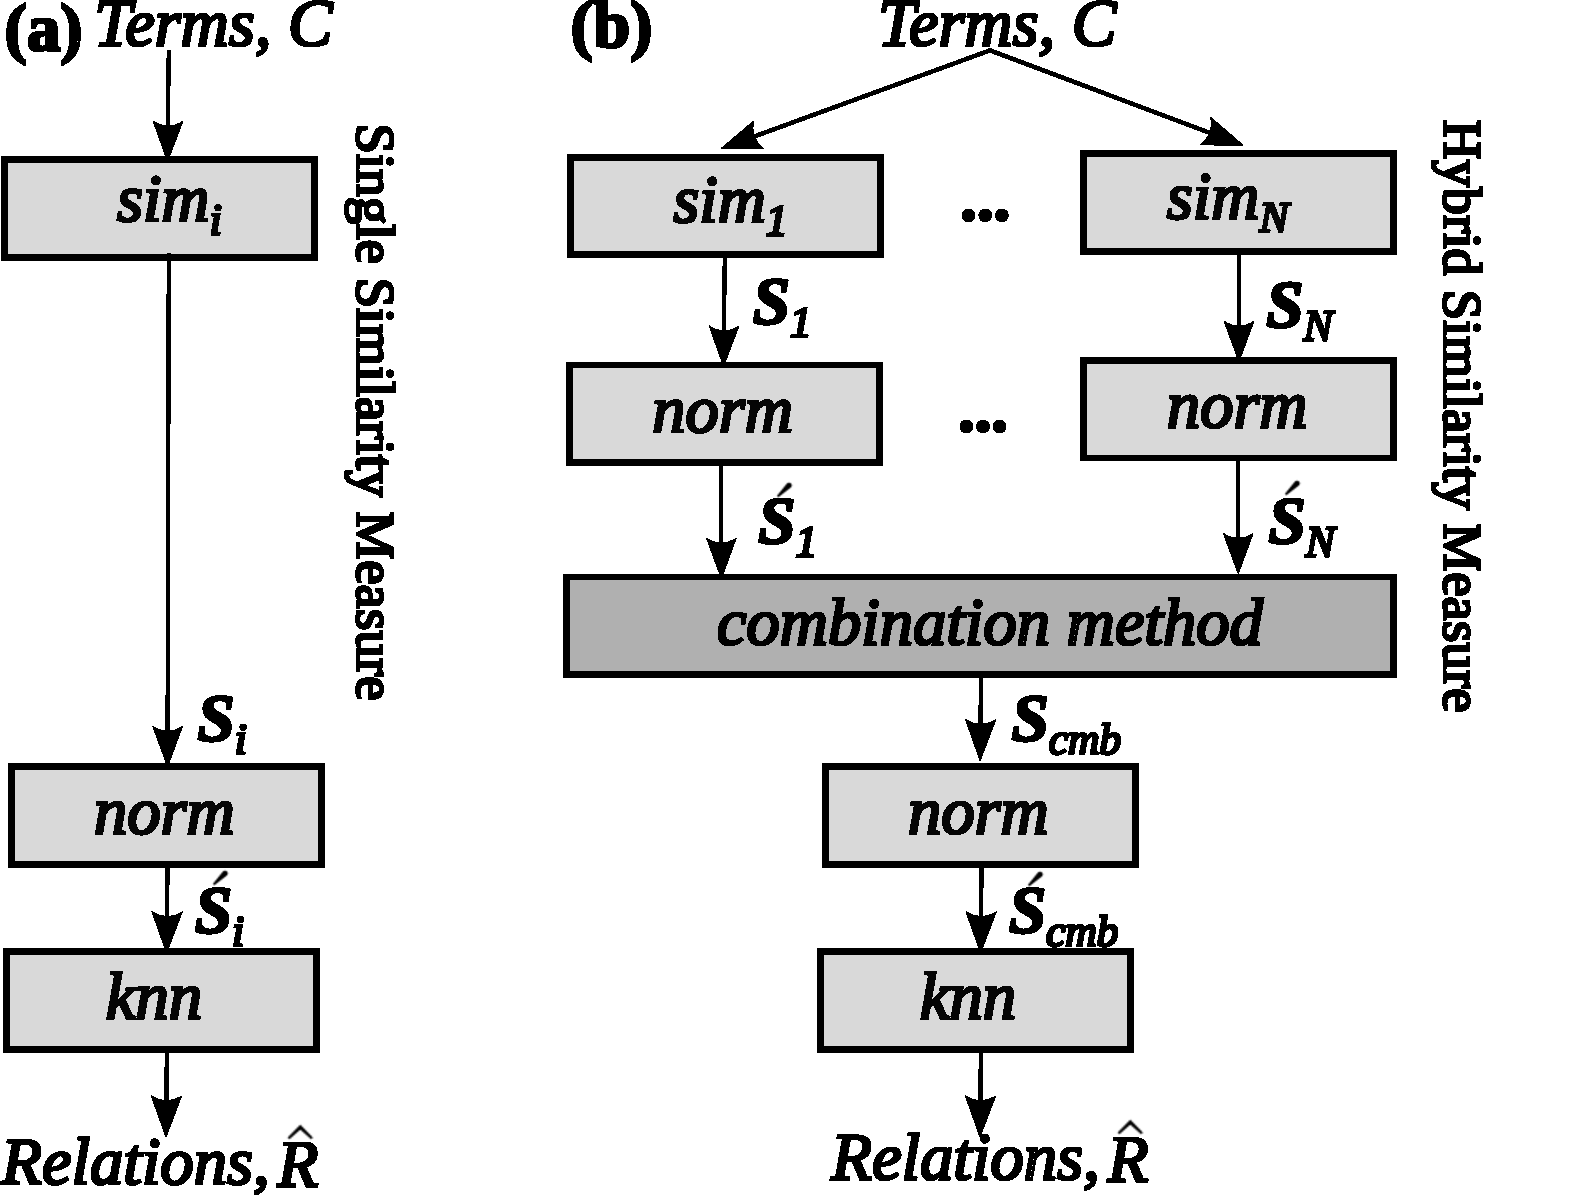
\includegraphics[width=0.65\textwidth]{figures/single-and-hybrid-2}
	\caption{Схема метода извлечения семантических отношений с помощью (а) отдельной метрики (b) комбинированной метрики.}		
\end{figure}


\end{frame}

\begin{frame}
\frametitle{Извлечение отношений на основе мер подобия}

\begin{block}{Метод}

\begin{algorithm}[H]
\SetLine
\KwIn{ Слова $C$,  Количество ближайших соседей $k$ }
\KwOut{ Семантические отношения $\hat{R} \subseteq C \times C  $ }

\For{i=1,N}{
$\mathbf{S}_i \leftarrow sim_i(C)$ \;
$\hat{\mathbf{S}}_{i} \leftarrow norm(\mathbf{S}_i)$ \;
}

$\mathbf{S}_{cmb} \leftarrow combination\_method(\hat{\mathbf{S}}_1,\ldots,\hat{\mathbf{S}}_N)$ \;

$\hat{\mathbf{S}}_{cmb} \leftarrow norm(\mathbf{S}_{cmb})$ \;
$\hat{R} \leftarrow knn(\hat{\mathbf{S}}_{cmb},k)$ \;
\Return{ $\hat{R}$ } \;
\label{alg:unsup}
\end{algorithm}

\end{block}
\end{frame}

\begin{frame}
\frametitle{Извлечение отношений на основе мер подобия}
\begin{itemize}
	\item $sim_i$ -- один из $N$ комбинируемых методов представленных в виде метрик.
	\item $norm$ -- нормализация $\hat{\mathbf{S}} = \frac{\mathbf{S}-min(\mathbf{S})}{max(\mathbf{S})}$	
	\item $knn$ -- алгоритм $k$ ближайших соседей:  $\hat{R}=\bigcup_{i=1}^{|C|}\left\{\left\langle c_i, c_j \right\rangle :  (c_j \in \text{ top }k\% \text{ of } c_i) \wedge (s_{ij} > 0) \right\}.$  

\item 34 отдельные метрики $sim$
\begin{itemize}
\item 13 основанные на \textbf{корпусе текстов} (дистрибутивный анализ, лексико-синтаксические шаблоны)
\item 9 основанные на \textbf{Веб-корпусе текстов}
\item 6 основанные на \textbf{семантической сети}
\item 6 основанные на \textbf{определениях} из словарей/энциклопедий    
\end{itemize}
\item 16 отдельные метрики были выбраны из 34 для комбинирования
\end{itemize}

\end{frame}


%%%%%%%%%%%%%%%%%%%%%%%%%%%%%%%%%%%%%%%%%%%%%%%%%
\begin{frame}
\frametitle{Метрики основанные на семантической сети}

 \textbf{Данные:} семантическая сеть WordNet 3.0, корпус SemCor.
	
 \textbf{Переменные:}
\begin{itemize}
\item $len(c_i,c_j)$ -- длина \textbf{кратчайшего пути} между $c_i$ и $c_j$
\item  $len(c_i, lcs(c_i,c_j))$ -- длина кратчайшего пути от $c_i$ до \textbf{ближайшего общего предка  (БОП)} слов $c_i$ и $c_j$
\item $len(c_{root}, lcs(c_i,c_j))$ -- длина кратчайшего пути от \textbf{корня} $c_{root}$ до БОП слов $c_i$ и $c_j$ (глубина БОП)
\item $P(c)$ --  \textbf{вероятность слова} $c$, оцененная из корпуса
\item  $P(lcs(c_i, c_j))$ -- \textbf{вероятность БОП} слов $c_i$ и $c_j$
\end{itemize}
	
 \textbf{Метрики:} Инвертированная длина пути (Jurafsky and Martin, 2009), Leacock-Chodorow (1998), Wu-Palmer (1994), 
 Resnik (1995), Jiang-Conrath (1997), Lin (1998).
  
\end{frame}

%%%%%%%%%%%%%%%%%%%%%%%%%%%%%%%%%%%%%%%%%%%%%%%%%
\begin{frame}
\frametitle{Метрики основанные на Веб корпусе текстов }

\textbf{Данные:} количество документов возвращенных ИПС (\textsc{Google, Yahoo, Yahoo BOSS, Bing}).
	
 \textbf{Переменные:} 
\begin{itemize}
	\item $h_i$ -- \textbf{количество документов} возвращенных по запросу слово $"c_i"$ 
	\item $h_{ij}$ -- \textbf{количество документов} возвращенных по запросу $"c_i \text{ AND } c_j"$
\end{itemize}

\textbf{Measures:} 
\begin{itemize}
\item Normalized Google Distance NGD (Cilibrasi and Vitanyi, 2007)
\item Pointwise Mutual Information PMI-IR (Turney, 2001)
\end{itemize}
\end{frame}

%%%%%%%%%%%%%%%%%%%%%%%%%%%%%%%%%%%%%%%%%%%%%%%%%
\begin{frame}
\frametitle{Метрики основанные на корпусе текстов}


\textbf{Данные:} корпус WaCkypedia (800M слов) и ukWaC (2000M токенов) 
	
\textbf{Переменные:} 
\begin{itemize}
  \item $\textbf{f}_i$-- вектор признаков представляющий слово $c_i$, основанный на \textbf{контекстном окне}
  \item $ \mathbf{f}^s_i$ -- вектор признаков представляющий слово $c_i$, основанный на \textbf{синтаксическом контекстном окне} 
\end{itemize}
	
\textbf{Метрики:}
\begin{itemize}
	\item Bag-of-word Distributional Analysis BDA (Sahlgren, 2006) 
	\item Syntactic Distributional Analysis SDA (Curran, 2003) 
 \end{itemize}
	
\textbf{Другие метрики}:
\begin{itemize}
\item Latent Semantic Analysis (LSA) на корпусе TASA (Landauer and Dumais, 1997)
\item NGD и PMI-IR на корпусе Factiva (Veksler et al., 2008)
\end{itemize}
	
\end{frame}




%%%%%%%%%%%%%%%%%%%%%%%%%%%%%%%%%%%%%%%%%%%%%%%%%
\begin{frame}
\frametitle{Метрики основанные на корпусе текстов }


	
Метрика основанная на \textbf{лексико-синтаксических шаблонах} 
\begin{itemize}
	\item \textbf{Данные} -- корпус WaCkypedia (800M слов) 
	\item 10 паттернов извлечения гиперонимов, ко-гиперонимов и синонимов:
	\item \texttt{such diverse \{[occupations]\} as
  \{[doctors]\}, \{[engineers]\} and \{[scientists]\}[PATTERN=1]}
  
  \item Сематническая близость между $c_i$ и $c_j$ пропорциональна количеству извлечений  $n_{ij}$ с помощью паттернов.
   $$
   sim(c_i,c_j) = \frac{n_{ij}}{max_{ij}(n_{ij})}.
   $$
\end{itemize}
 
 \end{frame}
 
 \begin{frame}
\frametitle{Метрики основанные на корпусе текстов }
	
Метрика основанная на \textbf{лексико-синтаксических шаблонах} 
 
 
 \begin{figure}
                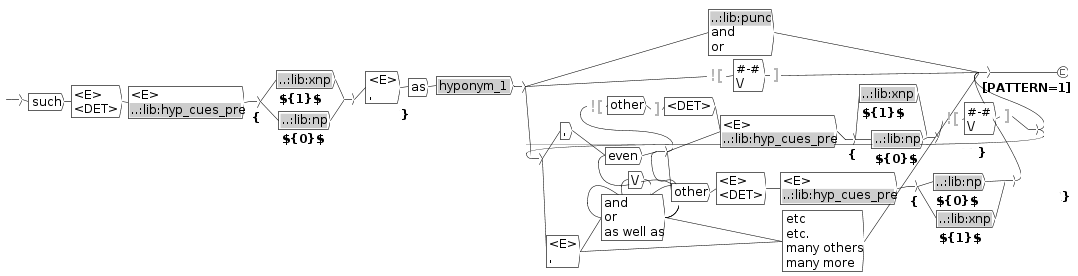
\includegraphics[width=1.0\textwidth]{figures/hypernym_1}
        \caption{Конечный автомат в формате \textsc{Unitex} для извлечения гиперонимов
        (под-автоматы обозначены серым цветом; <E> обозначает пустой символ; <DET> обозначает предлоги; полужирные символы -- аннотирующие тэги)}
        \label{fig:prcomb}
\end{figure}
	
\end{frame}




%%%%%%%%%%%%%%%%%%%%%%%%%%%%%%%%%%%%%%%%%%%%%%%%%
\begin{frame}
\frametitle{Метрики основанные на определениях}

\textbf{Данные:} определения WordNet, Wikipedia, и Wiktionary.
	
\textbf{Переменные:}
\begin{itemize}
		\item $gloss(c)$ -- \textbf{определение} слова
		\item $sim(gloss(c_i),gloss(c_j))$ -- \textbf{подобие слов} на основании их определений
		\item $\mathbf{f}_i$ -- \textbf{вектор признаков} слова $c_i$, вычисленный на корпусе из всех определений методов контекстного окна
		\item $\mathbf{f}_i$ \textbf{вектор признаков}, представляющий собой определение слова $c_i$
		\item $exist(c_i, c_j)$ связь между $c_i$ и $c_j$ в словаре
\end{itemize}

\textbf{Метрики:}
\begin{itemize}
  \item WktWiki -- BDA на определениях Wiktionary и Wikipedia
  \item ExtendedLesk на WordNet (Banerjee and Pedersen, 2003)
  \item GlossVectors на WordNet (Patwardhan and Pedersen, 2006)
\end{itemize}

\end{frame}


%%%%%%%%%%%%%%%%%%%%%%%%%%%%%%%%%%%%%%%%%%%%%%%%%
\begin{frame}
\frametitle{Метрики основанные на определениях  }

\begin{block}{Метрика WktWiki }
\begin{algorithm}[H]
\SetLine
\KwIn{ Слова $C$,  Количество признаков $\beta$}
\KwOut{ Матрица подобия, $\mathbf{S}$  $[C \times C]$ }

$D \leftarrow get\_wiktionary\_definitions(C)$ \;
$D \leftarrow D \cup get\_wikipedia\_definitions(C)$ \;
$\mathbf{F} \leftarrow construct\_fmatrix(C, D,  \beta)$ \;
$\mathbf{F} \leftarrow pmi(\mathbf{F}) $ \;
$\mathbf{S} \leftarrow cos(\mathbf{F})$ \;
$\mathbf{S} \leftarrow update\_similarity(\mathbf{S})$ \;
\Return $\mathbf{S}$ \;
\label{alg:wkt}
\end{algorithm}
\end{block}

\end{frame}



%%%%%%%%%%%%%%%%%%%%%%%%%%%%%%%%%%%%%%%%%%%%%%%%%
\begin{frame}
\frametitle{Методы комбинирования метрик подобия}
\begin{itemize}
\item Цель метода комбинирования метрик $combiation\_method$ -- более точно оценить семантическое подобие слов, на основе \textbf{информации из нескольких источников}.  

\item Метод комбинирования получает на вход множество матриц подобия $\{\mathbf{S}_1,\ldots,\mathbf{S}_K\}$ сгенерированных $K$ метриками и возвращает комбинированную матрицу подобия $\mathbf{S}_{cmb}$. 

\item Здесь  $s_{ij}^k$ -- \textbf{семантическое подобие слов} $c_i$ и $c_j$ согласно $k$-ой метрике $sim_k$. 

\item Мы используем 8 методов комбинирования метрик.

\end{itemize}
\end{frame}

\begin{frame}
\frametitle{Методы комбинирования метрик подобия}

\begin{enumerate}
  
\item \textbf{Mean}. Среднее  между значениями подобия метрик:
$$\mathbf{S}_{cmb} = \frac{1}{K} \sum_{k=1}^K \mathbf{S}_k \Leftrightarrow 
s_{ij}^{cmb}= \frac{1}{K}\sum_{k=1,K} s_{ij}^k.$$

\item \textbf{Mean-Nnz}. Среднее между ненулевыми значениями подобия: $$s_{ij}^{cmb}= \frac{1}{|k:s_{ij}^k
>0,k=1,K|}\sum_{k=1,K} s_{ij}^k.$$

\item \textbf{Mean-Zscore}. Среднее  между стандартизированными значениями подобия метрик:
$$\mathbf{S}_{cmb} = \frac{1}{K} \sum_{k=1}^K \frac{\mathbf{S}_k -
\mu_k}{\sigma_k},$$ где $\mu_k$ и $\sigma_k$ -- среднее и стандартное отклонение значений подобия $k$-ой метрики ($\mathbf{S}_k$).

\end{enumerate}
\end{frame}



\begin{frame}
\frametitle{Методы комбинирования метрик подобия}

\begin{enumerate}
  \setcounter{enumi}{3}
\item \textbf{Median}. Медиана значений подобия метрик:
$$s_{ij}^{cmb}= median(s_{ij}^1,\ldots,s_{ij}^K). $$

\item \textbf{Max}. Максимальное значение из значений подобия метрик:
$$s_{ij}^{cmb}= max(s_{ij}^1,\ldots,s_{ij}^K).$$

\item \textbf{RankFusion}.Среднее значение ранга пары слов:
 $$s_{ij}^{cmb}= \frac{1}{K}\sum_{k=1,K}
r_{ij}^k,$$
где $r^k_{ij}$ -- ранг, соответствующий значению подобия $s^k_{ij}$.
\end{enumerate}

\end{frame}



\begin{frame}
\frametitle{Методы комбинирования метрик подобия}

\begin{enumerate}
  \setcounter{enumi}{6}
  \item \textbf{RelationFusion}. Идея -- объединить лучшие отношения найденные каждым методом. При этом   отношения извлеченные несколькими методами -- лучше. 

\begin{algorithm}[H]
\SetLine
\KwIn{Матрицы подобия сгенерированные $N$ базовыми метриками $\{\mathbf{S}_1,\ldots,\mathbf{S}_N\}$, количество ближайших соседей $k$}
\KwOut{ Комбинированная матрица подобия, $\mathbf{S}_{cmb}$  }

\For{i=1,N}{$R_i \leftarrow knn(\mathbf{S}_i, k)$ \;
 $\mathbf{R}_i \leftarrow relation\_matrix(R_i)$}
$\mathbf{S}_{cmb} \leftarrow \frac{1}{N} \sum_{i=1}^N \mathbf{R}_i$ \;
\Return $\mathbf{S}_{cmb}$ \;
\label{rfusion}
\end{algorithm}
$$
r_{ij} = \left\{ 
  \begin{array}{l l}
    1 & \quad \text{if } \langle c_i, t, c_j \rangle \in R_k \\
    0 & \quad \text{else}\\
  \end{array} \right.
$$

\end{enumerate}

\end{frame}


\begin{frame}
\frametitle{Методы комбинирования метрик подобия}

\begin{enumerate}
  \setcounter{enumi}{7}
\item \textbf{Logit}. 
 Метод основан на обучении с учителем и использует \textbf{Логистическую регрессию} (Agresti, 2002). 

\begin{enumerate}
  \item Обучение бинарного классификатора на множестве пар семантически связных и несвязных слов BLESS and SN 
  \item Отношение $\langle c_i, t, c_j \rangle$ представлено в виде $K$-мерного вектора из 
значений подобия $(s_{ij}^1,\ldots,s_{ij}^K)$ 

\item Целевая переменная $r_{ij}$ (категория):
$$
r_{ij} = \left\{ 
  \begin{array}{l l}
    0 & \quad  \text{ тип отношения } t = random
    \\
    1 & \quad  \text{ иначе }\\
  \end{array} \right
  .
$$

\item Применение модели для комбинирования метрик: 
$$\mathbf{S}_{cmb} = \frac{1}{1 + e^{-z}}, z = w_0 + \sum_{k=1}^K w_k \mathbf{S}_k , $$

где $K+1$ коэффециента $(w_0, w_1,\ldots, w_K)$ -- веса регрессии полученные в результате обучения.
 \end{enumerate}
\end{enumerate}

\end{frame}

%%%%%%%%%%%%%%%%%%%%%%%%%%%%%%%%%%%%%%%%%%%%%%%%%
\begin{frame}
\frametitle{Какие из отдельных метрик следует комбинировать?}

\begin{itemize}
\item Количество \textbf{возможных комбинаций}:
 $\sum_{m=2}^{34}C_{34}^m=\sum_{m=2}^{34}\frac{34!}{m!(34-m)!}=1.718 \cdot 10^{10}$
 
$\sum_{m=2}^{16}C_{16}^m=\sum_{m=2}^{16}\frac{16!}{m!(16-m)!}=65535$
 
\item \textbf{Экспертный выбор} -- 5, 9 и 15 метрик из 16
\item \textbf{Forward Stepwise Procedure} -- 7,8a,8b,10 метрик из 16
\item Анализ коэффициентов \textbf{Логистической регрессии} -- 12 из 16

%\begin{itemize}
 %\item \textbf{5} % = WN-Resnik, BDA-3-5000, SDA-21-100000,  Def-WktWiki-1000
 %\item \textbf{9} %= \textbf{Group4} + WN-WuPalmer, LSA-Tasa, Def-GlossVec., and Def-Ext.Les
 %\item \textbf{15} %= \textbf{Group8} + WN-LeacockChodorow, WN-Lin, WN-JiangConrath, NGD-Factiva, NGD-Yahoo, and NGD-GoogleWiki.
%\end{itemize}

\end{itemize}
\end{frame}
  

%%%%%%%%%%%%%%%%%%%%%%%%%%%%%%%%%%%%%%%%%%%%%%%%%
\section{Критерии}


%%%%%%%%%%%%%%%%%%%%%%%%%%%%%%%%%%%%%%%%%%%%%%%%%
\begin{frame}
\frametitle{Критерии основанные на суждениях субъектов о семантической связанности}

\begin{table}[h]\footnotesize
\begin{tabular}{ |c|c|c|c|c|c| }
\hline
  слово, $c_i$ & слово, $c_j$ & субъект, $\mathbf{s}$  & sim, $\mathbf{s}$  & субъект (ранг), $\mathbf{r}$ & sim (ранг), $\hat{\mathbf{r}}$  \\ \hline \hline
tiger & cat & 7.35 & 0.85 & 1 & 3 \\
book & paper & 7.46 &  0.95 & 2 & 2 \\
computer & keyboard & 7.62 &  0.81 & 3 & 1 \\
... & ... & ... & ...   & \ldots & \ldots \\
possibility & girl & 1.94 & 0.25 & 64 & 65 \\
sugar & approach & 0.88 & 0.05 & 65 & 23 \\ \hline
\end{tabular}
\end{table}


\textbf{Данные:}

\begin{itemize}
	\item WordSim353 -- 353 пар слов (Finkelstein, 2002)  
	\item MC -- 30 пар слов  (Miller & Charles, 1991)
	\item RG -- 65 пар слов (Rubenstein & Goodenough, 1965)  
\end{itemize}

\textbf{Коэффициент корреляции Пирсона:}  $\rho = \frac{cov(\mathbf{s},\hat{\mathbf{s}})}{\sigma(\mathbf{s}) \sigma(\hat{\mathbf{s}})}$

 \textbf{Коэффициент корреляции Спирмена:}: $r = \frac{cov(\mathbf{r},\hat{\mathbf{r}})}{\sigma(\mathbf{r}) \sigma(\hat{\mathbf{r}})}$
 
\end{frame}


%%%%%%%%%%%%%%%%%%%%%%%%%%%%%%%%%%%%%%%%%%%%%%%%%
\begin{frame}
\frametitle{Критерии точности извлечения отношений}

{ \scriptsize

\begin{table}[h]\footnotesize
\begin{tabular}{ |c|l|l| }
\hline
\bf слово, $c_i$ & \bf  слово, $c_j$ & \bf тип отношения, $t$  \\ \hline \hline
judge & adjudicate & syn \\
judge & arbitrate & syn \\
judge & asessor & syn \\
judge & chancellor & syn \\
judge & gendarmerie & syn \\
judge & sheriff & syn \\
... & ... & ...   \\
judge & pc & random \\ 
judge & fare & random \\
judge & lemon & random \\ \hline
\end{tabular}
\end {table}

}

\textbf{Данные:}
\begin{itemize}
  \item BLESS (Baroni and Lenci, 2011)	-- 26554 отношений (hyper, coord, mero, event, attri, random)  
  \item SN (Panchenko, 2012) -- 14682  отношений (syn, random) 
\end{itemize}

\end{frame}

%%%%%%%%%%%%%%%%%%%%%%%%%%%%%%%%%%%%%%%%%%%%%%%%%
\begin{frame}
\frametitle{Критерии точности извлечения отношений}

\begin{itemize}
  
  \item Основаны на количестве правильно извлеченных отношений.
  

\item $R$ -- все семантические отношения, не являющиеся случайными ($\langle animal, random, bishop \rangle$ и т.п.)

\item $\hat{R}(k)$ множество извлеченных отношений при количестве ближайших соседей $k$

\begin{block}{Критерии}

	
	\begin{itemize}
		\item Точность: $P(k)=$$\frac{|R \cap \hat{R}(k)|}{|\hat{R}(k)|}$,
		\item Полнота: $R(k)=$$\frac{|R \cap \hat{R}(k)|}{|R|}$,
		\item F1-мера: $F(k)= 2 \cdot \frac{P(k) \cdot R(k)}{P(k) + R(k)}$,
		\item MAP $M(k) = \frac{1}{k}\sum^{k}_{i=1}P(i)$.
	\end{itemize}	
	\end{block}

\item Мы используем $P(10)$, $P(20)$, $P(50)$, $R(50),MAP(20)$, $MAP(50)$.
	

\end{itemize}
	
	
\end{frame}


%%%%%%%%%%%%%%%%%%%%%%%%%%%%%%%%%%%%%%%%%%%%%%%%%
\begin{frame}
\frametitle{Пример: оценка точности извлечения отношений}

\begin{itemize}
	\item Точность $P(50\%)= \frac{1}{7} \approx 0.86 $
\end{itemize}


\begin{table}[h]\footnotesize
\begin{tabular}{ |l|l|l|l| }
\hline
\bf слово, $c_i$ & \bf  слово, $c_j$ & \bf тип отношения & \bf $s_{ij}$ \\ \hline \hline

aficionado & enthusiast & syn & 0.07197 \\
aficionado & fan & syn & 0.05195 \\
aficionado & admirer & syn & 0.01964 \\
aficionado & addict & syn & 0.01326 \\
aficionado & devotee & syn & 0.01163 \\
aficionado & foundling & random & 0.00777 \\
aficionado & fanatic & syn & 0.00414 \\ \hline
aficionado & adherent & syn & 0.00353 \\
aficionado & capital & random & 0.00232 \\
aficionado & statute & random & 0.00029 \\
aficionado & blot & random & 0.00025 \\
aficionado & meddler & random & 0.00005 \\
aficionado & enlargement & random &	0.00003 \\
aficionado & bawdyhouse & random & 	0.00000 \\ 
\hline
\end{tabular}
\end {table}

\end{frame}

\section{Результаты}

\begin{frame}
\frametitle{Отдельные метрики: корреляция с суждениями субъектов}

	\begin{figure}
	\centering
		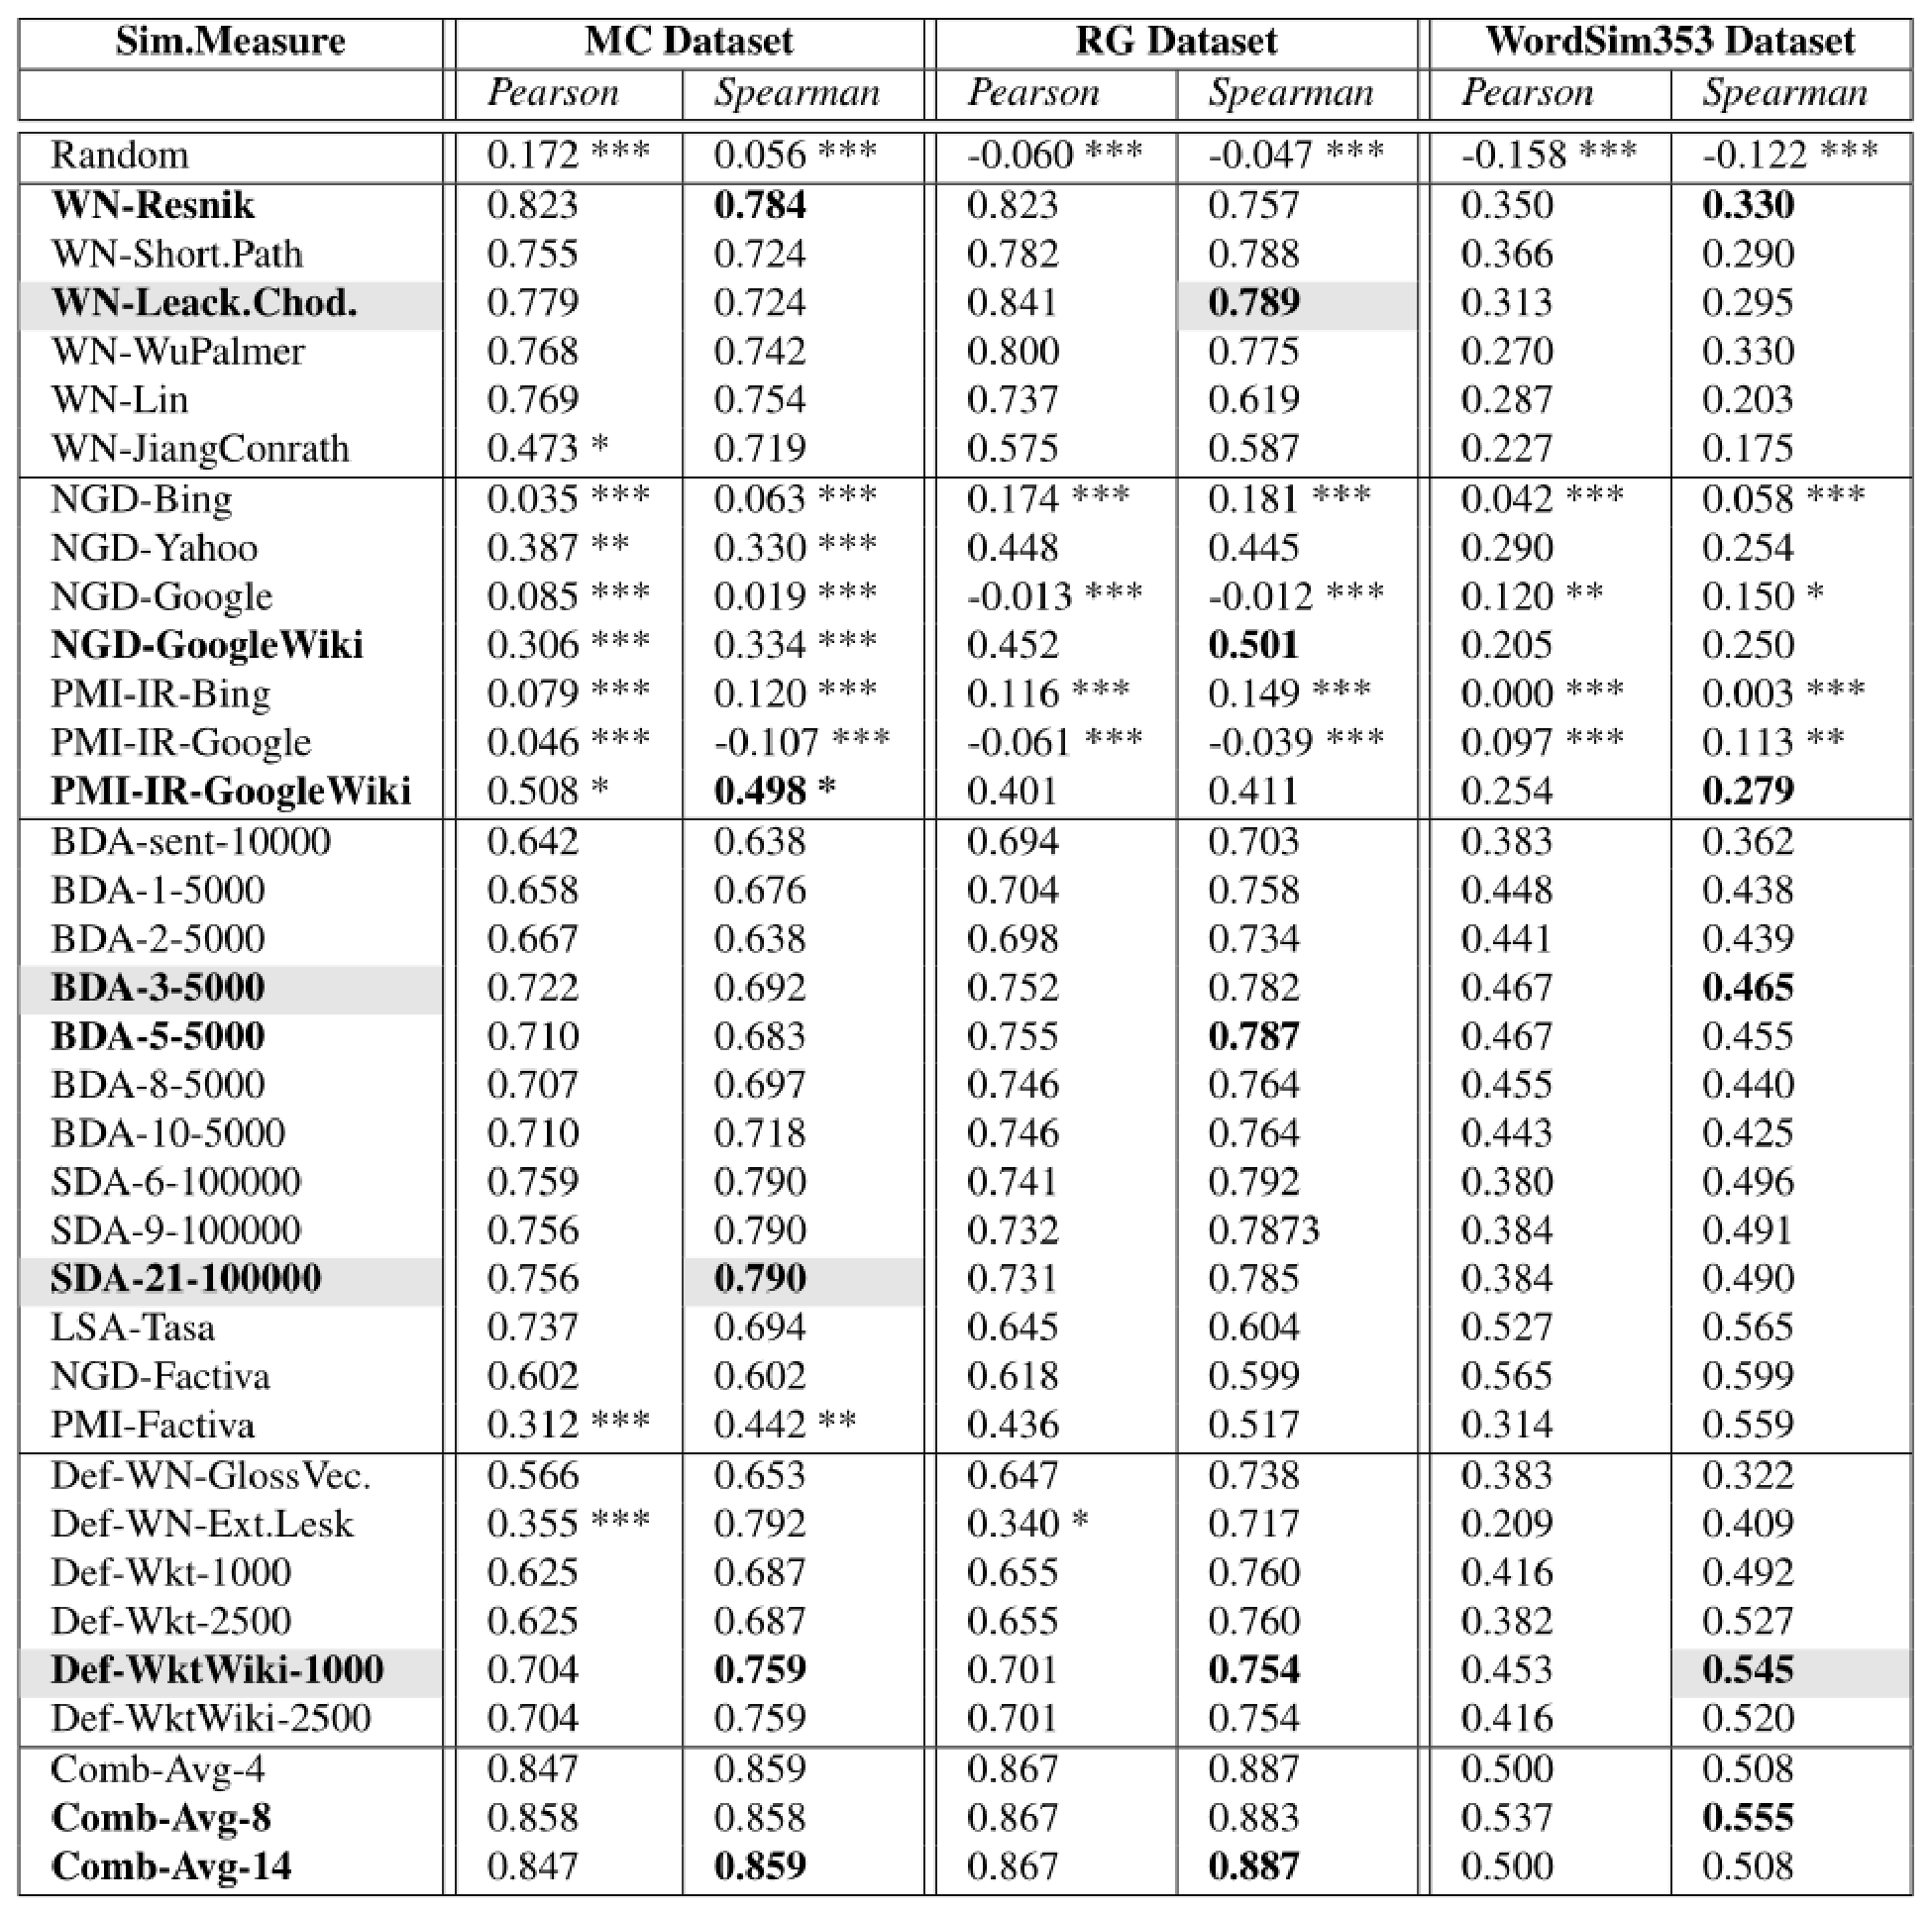
\includegraphics[width=0.62\textwidth]{figures/hj}
		\caption{\footnotesize Pearson -- корреляция Пирсона, Spearman -- корреляция Спирмена.}
		
\end{figure}
	
\end{frame}

%%%%%%%%%%%%%%%%%%%%%%%%%%%%%%%%%%%%%%%%%%%%%%%%%
\begin{frame}
\frametitle{Отдельные метрики: извлечение отношений}

	\begin{figure}
	\centering
		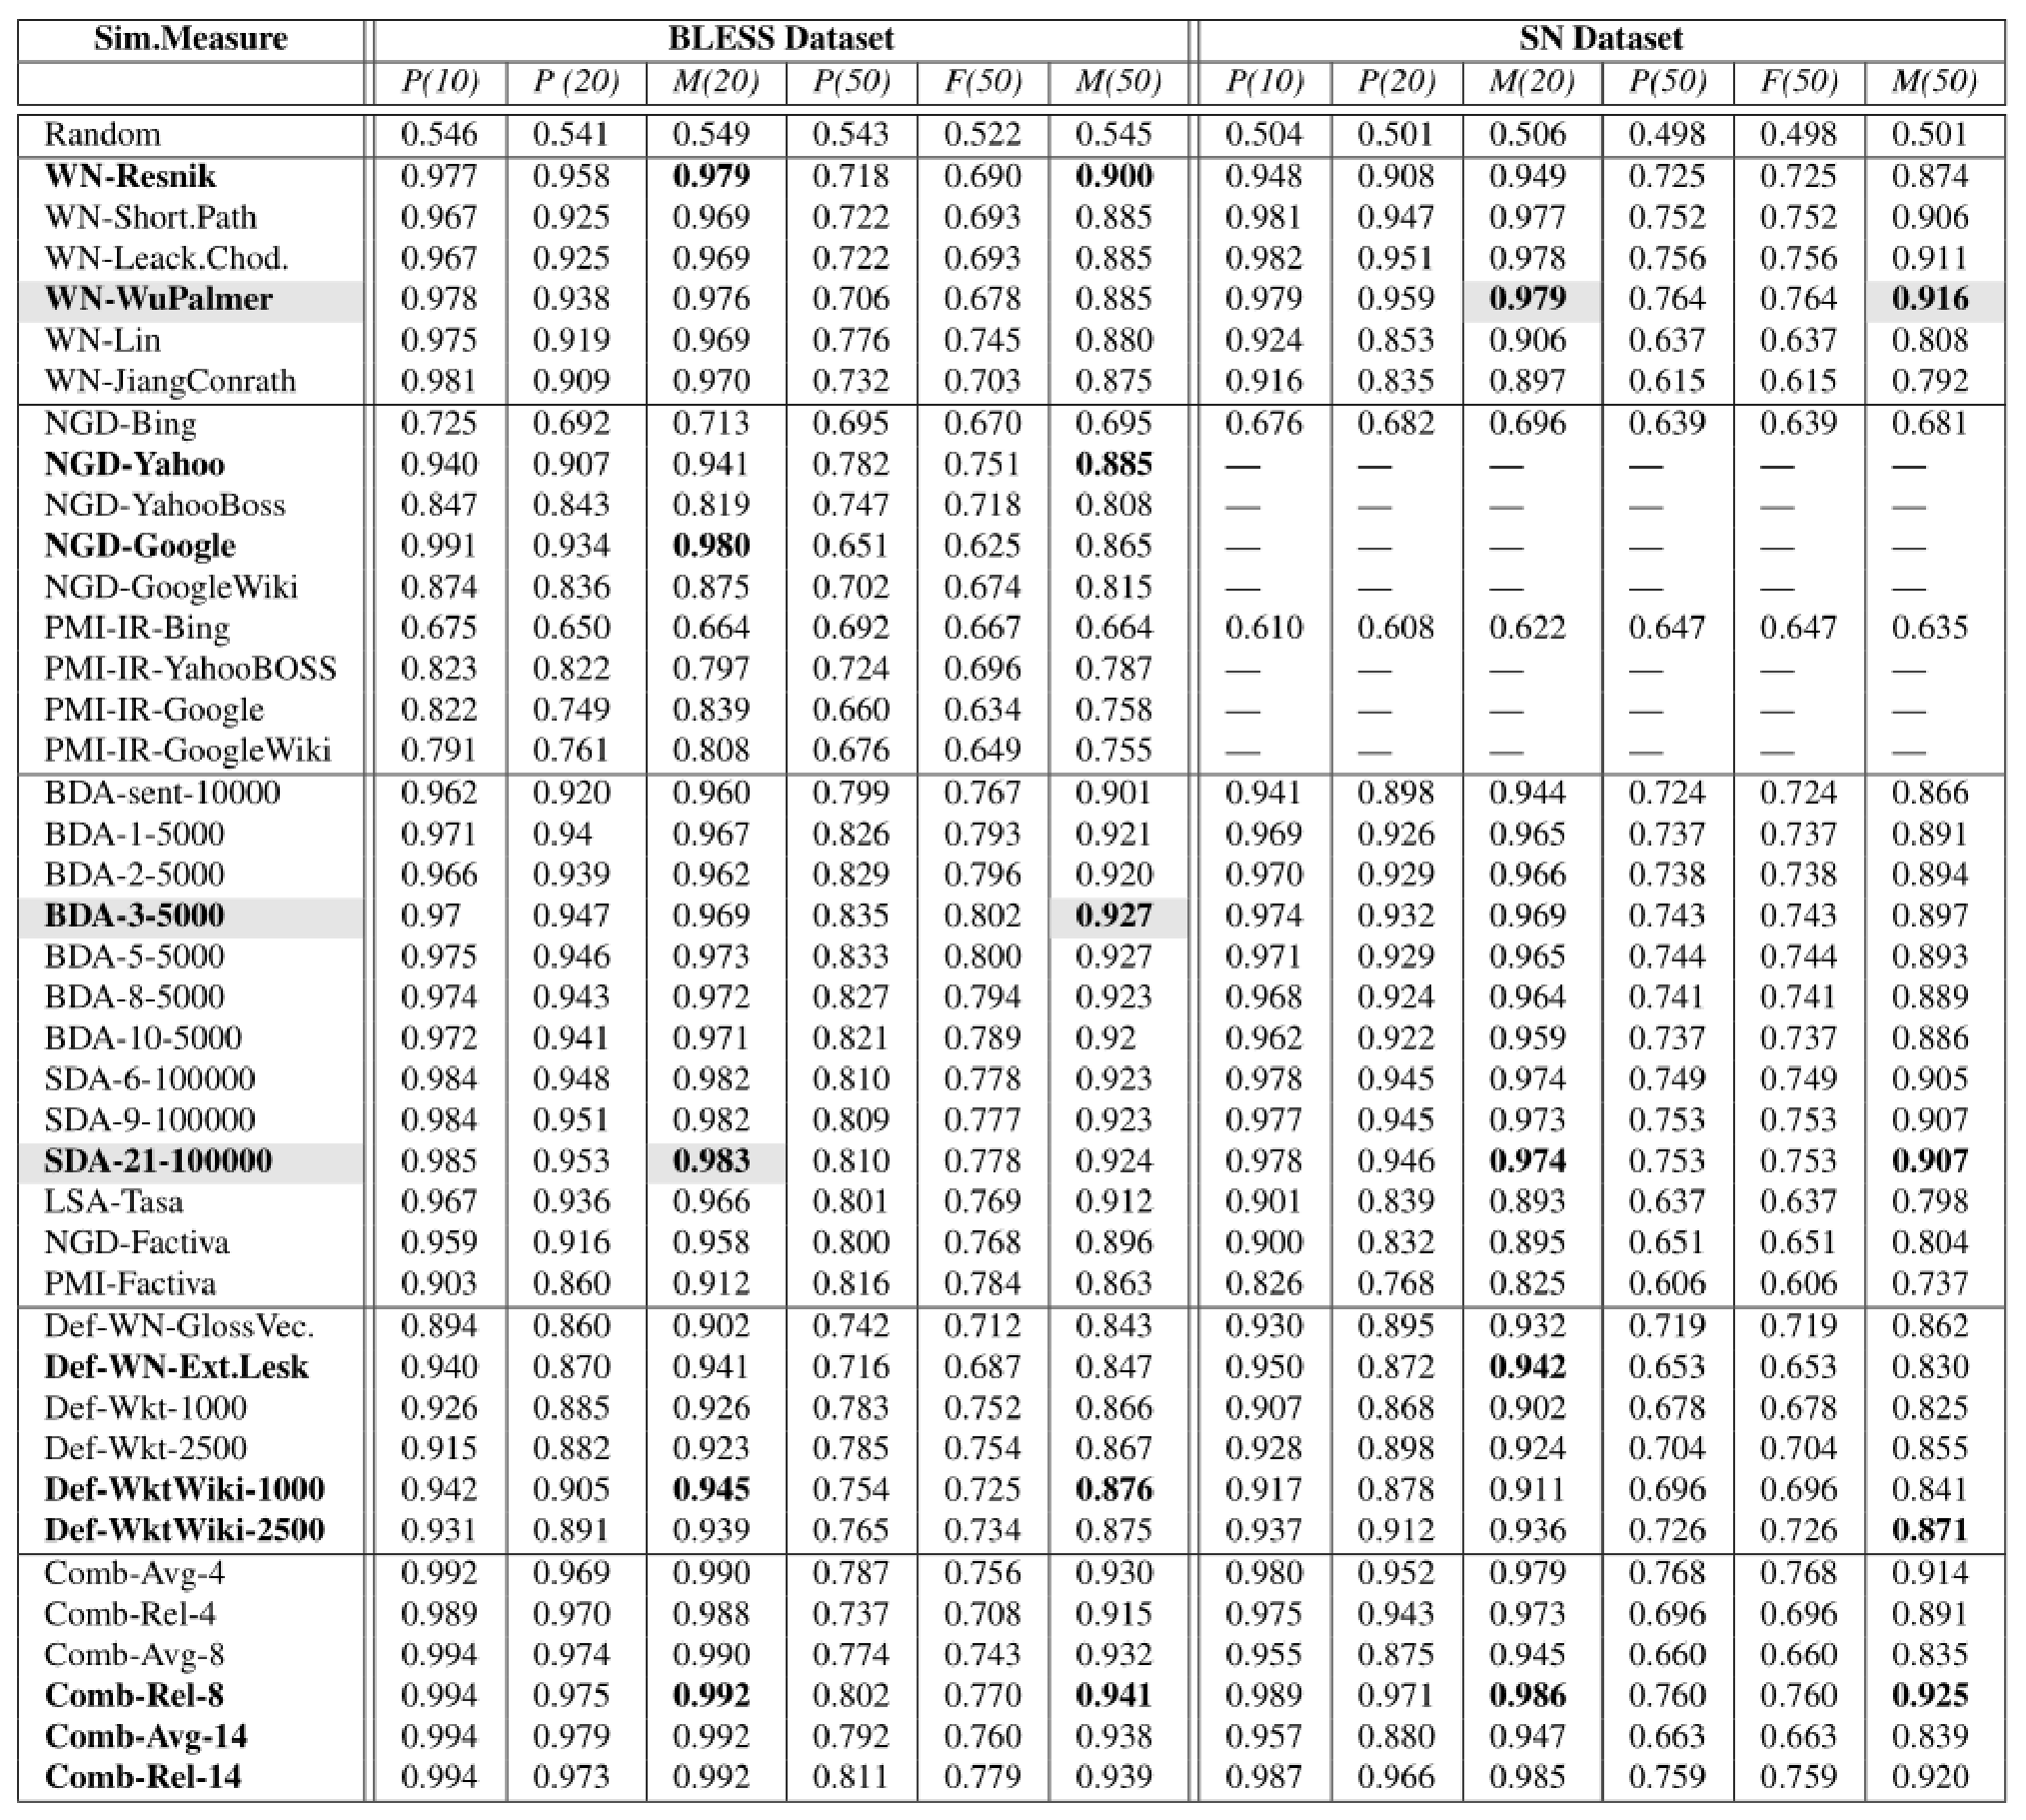
\includegraphics[width=0.65\textwidth]{figures/sr}
		\caption{Здесь P -- точность, R -- полнота, F -- F1-мера, M -- MAP.}
		
\end{figure}
	
\end{frame}

%%%%%%%%%%%%%%%%%%%%%%%%%%%%%%%%%%%%%%%%%%%%%%%%%
\begin{frame}
\frametitle{Отдельные метрики }

	\begin{figure}
	\centering
		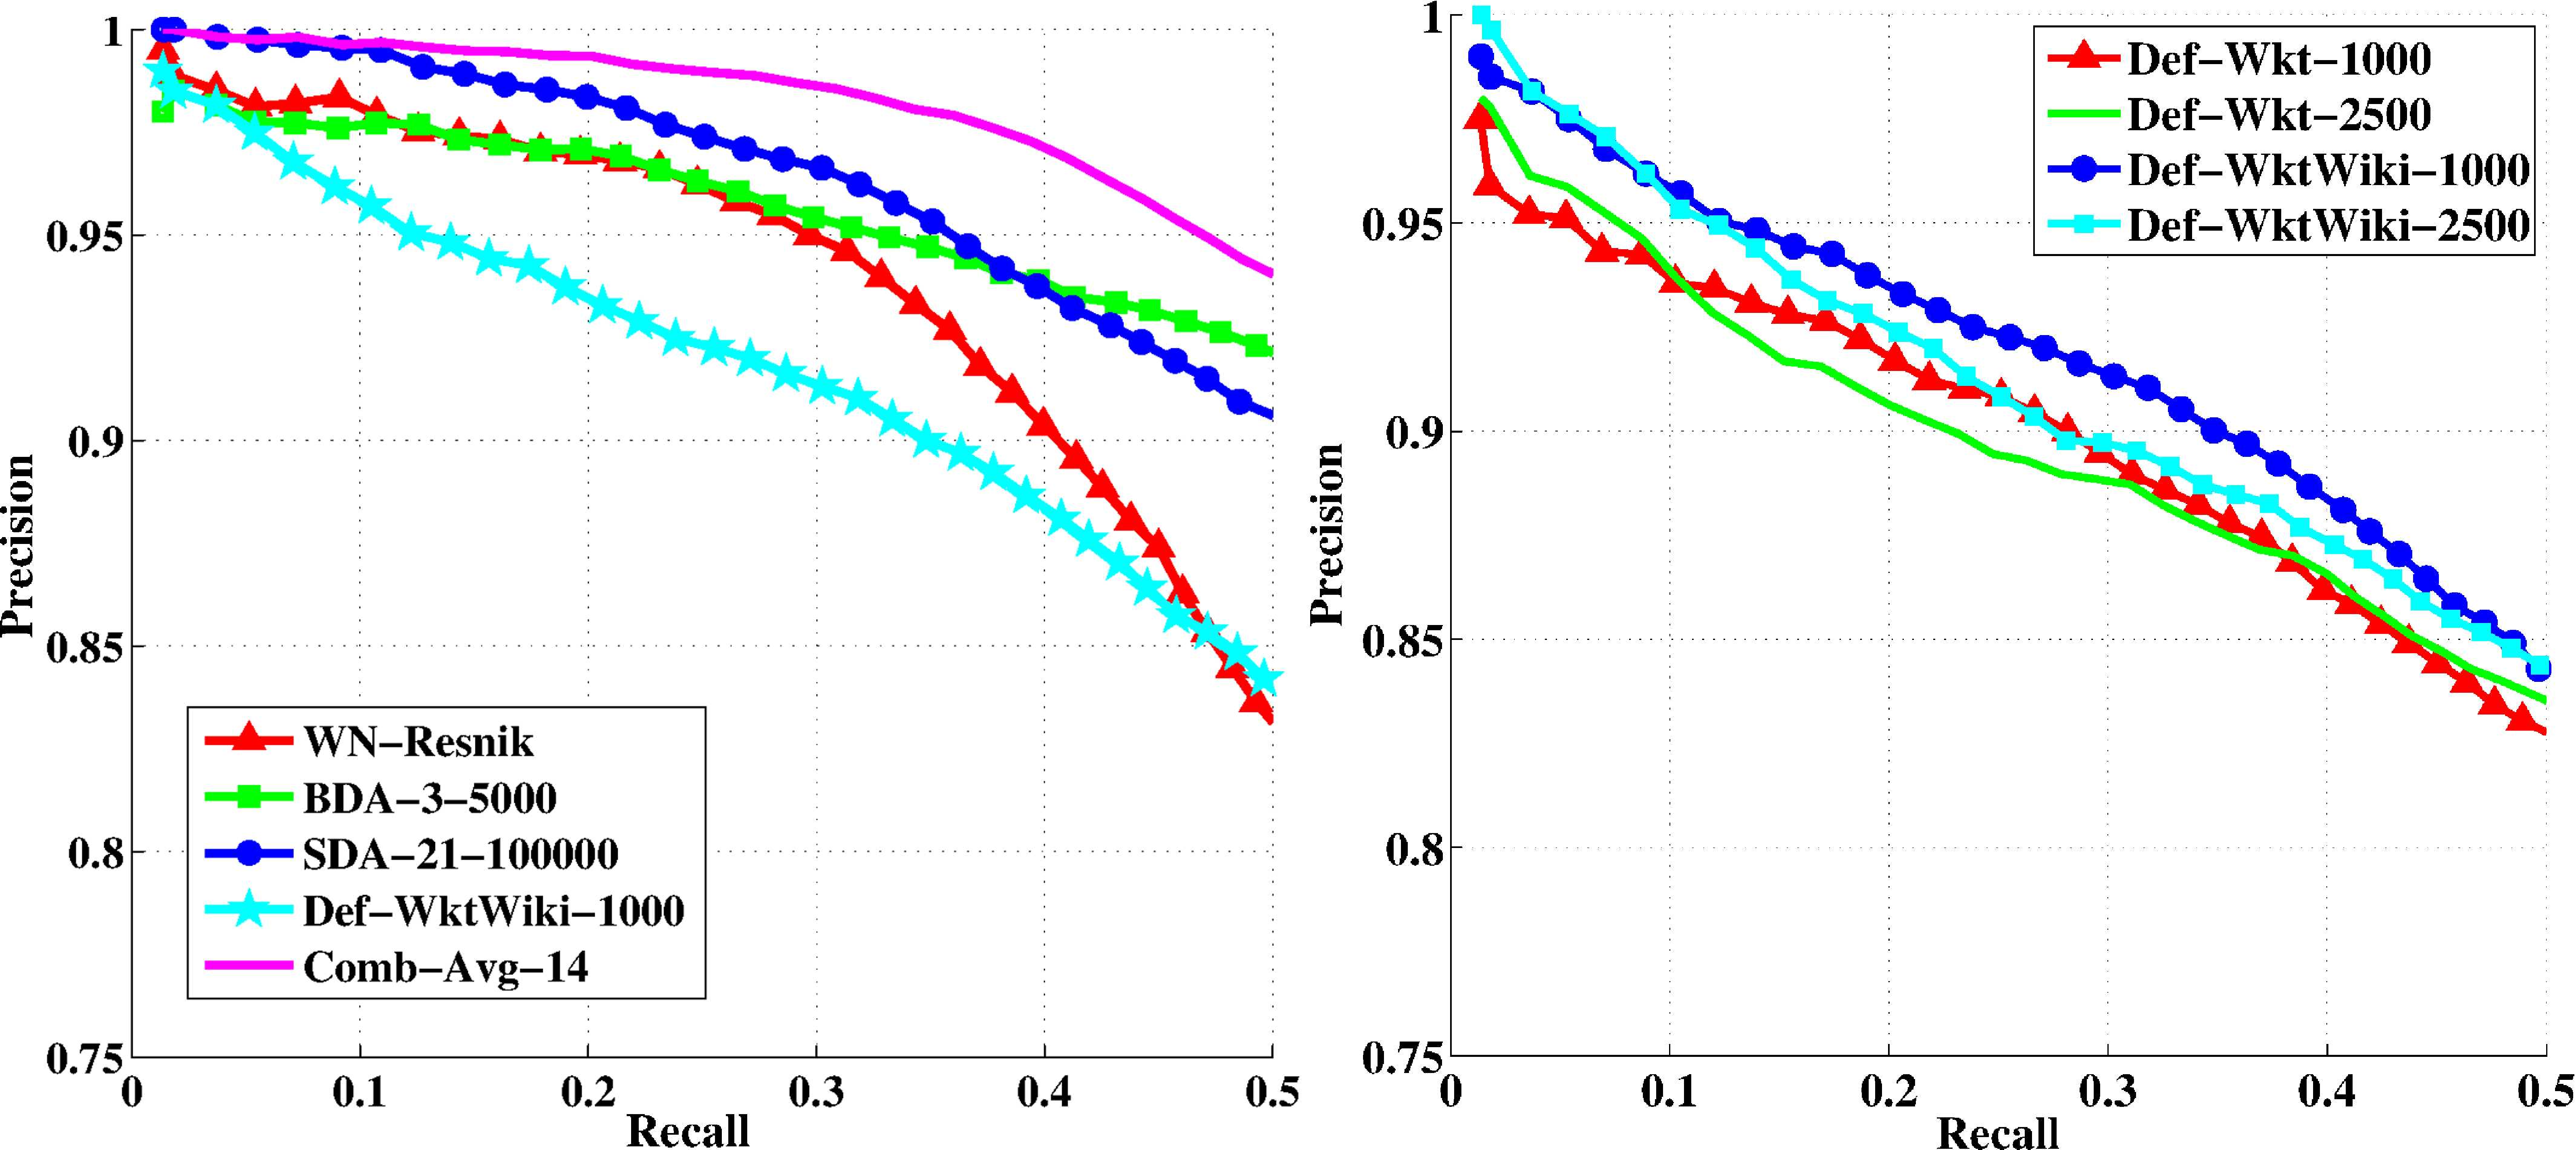
\includegraphics[width=1.0\textwidth]{figures/pr-plots-2}
			\caption{Графики Точность-Полнота (слева) 4х лучших метрик основанных на корпусе, семантических сетях, определениях и метрика, основанная на среднем значении 14 метрик; (слева) метрики основанных на определениях Викисловаря и Википедии. }
\end{figure}
	
\end{frame}


%%%%%%%%%%%%%%%%%%%%%%%%%%%%%%%%%%%%%%%%%%%%%%%%%
\begin{frame}
\frametitle{Отдельные и комбинированные метрики }


	\begin{figure}
	\centering
		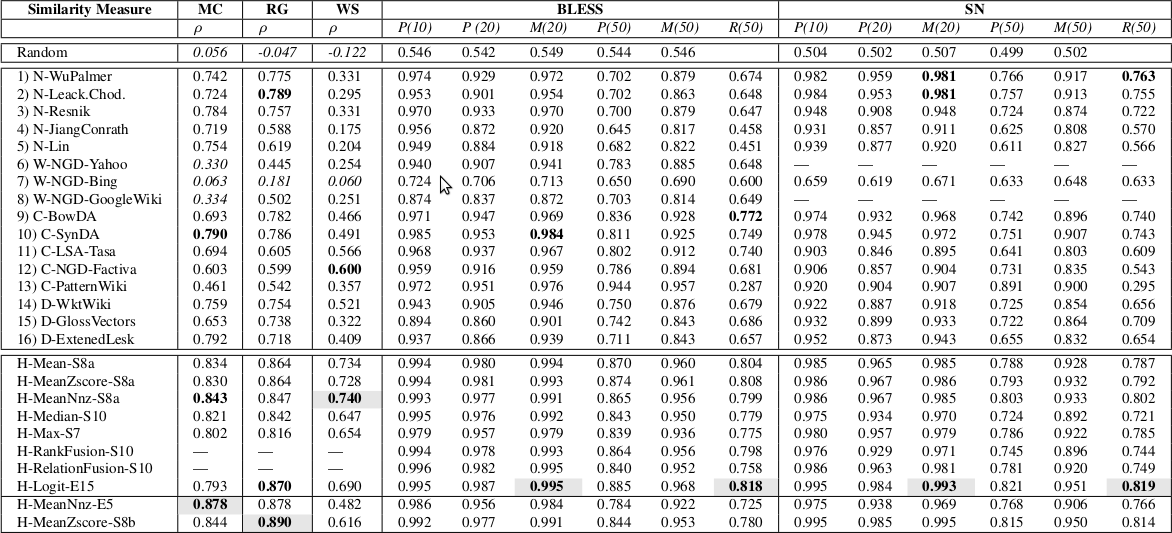
\includegraphics[width=1.0\textwidth]{figures/table-hybrid}
		\caption{
		\footnotesize
		Характеристики 16 отдельных и 8 комбинированных метрик. MC, RG, WordSim353 -- корреляция с суждениями человека. BLESS, SN -- точность извлечения семантических отношений. Наилучшие значения в группе (отдельные/комбинированные) обозначены полужирным шрифтом; наилучшие значения  обозначены серым цветом. Статистически незначимые корреляции (p > 0.05) обозначены курсивом, иначе $p \leq 0.05$.}
\end{figure}
	
\end{frame}

%%%%%%%%%%%%%%%%%%%%%%%%%%%%%%%%%%%%%%%%%%%%%%%%%
\begin{frame}
\frametitle{ Отдельные и комбинированные метрики }


	\begin{figure}
	\centering
		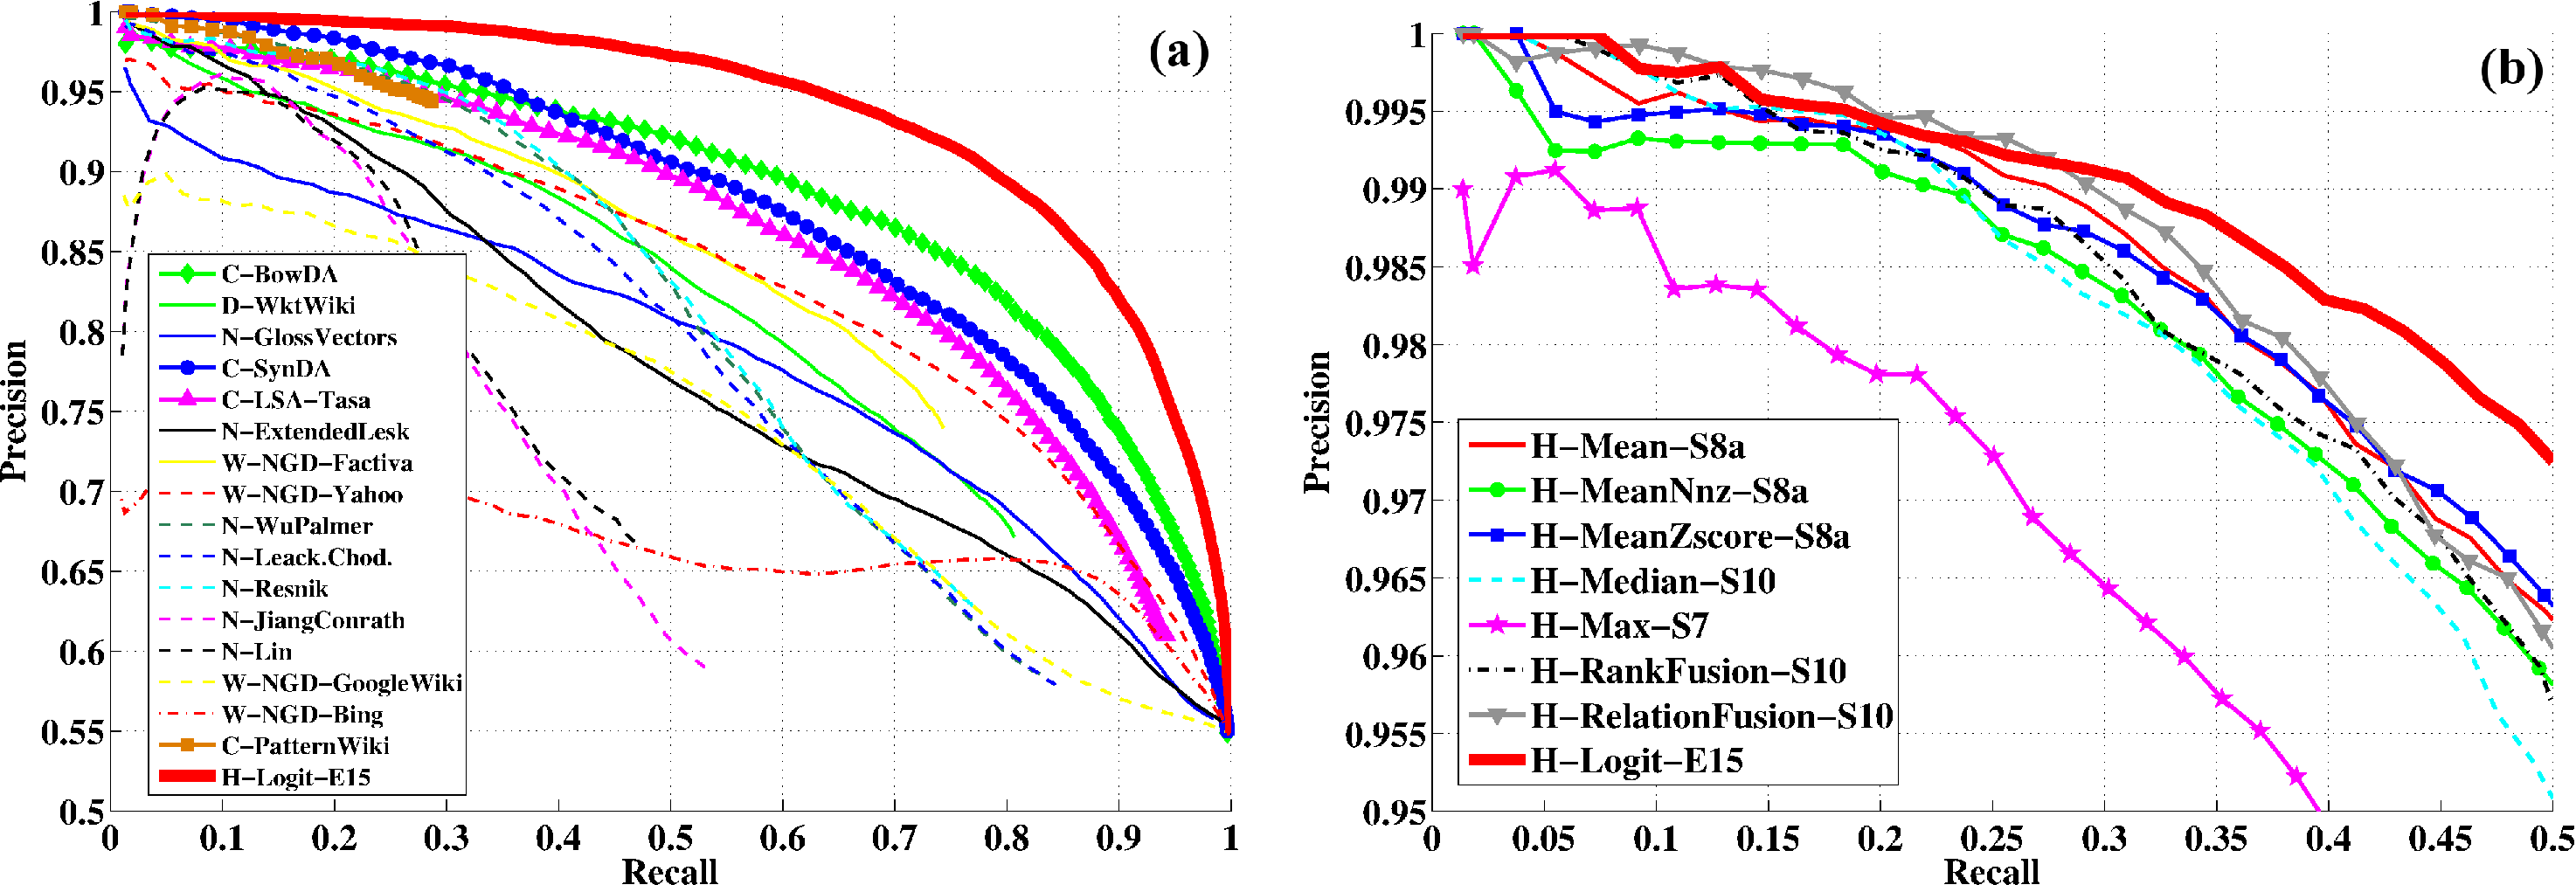
\includegraphics[width=1.0\textwidth]{figures/pr}
		\caption{График Точность-Полнота на множестве отношений BLESS для (a) 16
                отдельных метрик и лучшей комбирированной метрике H-Logit-E15; (b) 8 комбинированных метрик.
}
\end{figure}
	
\end{frame}

%%%%%%%%%%%%%%%%%%%%%%%%%%%%%%%%%%%%%%%%%%%%%%%%%
\section{Заключение}


%%%%%%%%%%%%%%%%%%%%%%%%%%%%%%%%%%%%%%%%%%%%%%%%%
\begin{frame}
\frametitle{Заключение:}

\begin{block}{Новизна работы:}
\begin{enumerate}
\item Сравнение 34 базовых метрик семантического подобия на задаче извлечения семантических отношений.   
\item Разработка и сравнительный анализ 8 комбинированных методов извлечения отношений.
\item Предложенный комбинированный метод H-Logit-E15, основанный на логистической регрессии:
	\begin{itemize}
	\item превосходит все отдельные и комбинированные методы;
 	\item достигает корреляции с суждениями человека до 0.870;
 	\item достигает MAP(20) при извлечения отношений до 0.995.
	\end{itemize}   
\end{enumerate}
\end{block}

\end{frame}

%%%%%%%%%%%%%%%%%%%%%%%%%%%%%%%%%%%%%%%%%%%%%%%%%
\begin{frame}
\frametitle{Текущие исследования:}

\begin{block}{Более сложные методы комбинирования:}	
\begin{itemize}
	\item Комбинирование с учителем -- \textbf{машины опорных векторов SVM} (Вапник, 1992)
	\item Комбинирование без учителя -- \textbf{методы факторизации разряженных тензоров PARAFAC, NTF} (Colda, 2004)   
\end{itemize}
\end{block}

\begin{block}{Приложения метода:}	
\begin{itemize} 
			\item В модуле расширения поискового запроса в платформе извлечения информации Biographe
			\item В модуле классификации имен файлов в системе мониторинга P2P сетей iCOP
			\item Для построения лексико-семантической поисковой системы LSSE
\end{itemize}
\end{block}


\end{frame}

\end{document}